\documentclass[12pt,a4paper]{article}
\usepackage[utf8]{inputenc}
\usepackage[russian]{babel}
\usepackage[OT1]{fontenc}
\usepackage{mathtools}
\usepackage{amsfonts}
\usepackage{amssymb}
\usepackage{enumitem}
\usepackage{alltt}
\usepackage{graphicx}
\usepackage{indentfirst}
\usepackage{caption}
\usepackage{float}
\usepackage{wrapfig}
\usepackage{physics}
\usepackage{multirow}
\usepackage{longtable}
\usepackage{amsmath,amsfonts,amssymb,amsthm,mathtools}
\usepackage{icomma}
\setlength{\parindent}{0.75cm}
\graphicspath{{pictures/}}
\DeclareGraphicsExtensions{.png, .jpg}
\usepackage[left=15mm,right=15mm,top=2cm,bottom=2cm]{geometry}
\author{Глотов Алексей}
\begin{document}
\newpage
\begin{center}
\footnotesize{{ГОСУДАРСТВЕННОЕ АВТОНОМНОЕ ОБРАЗОВАТЕЛЬНОЕ УЧРЕЖДЕНИЕ}\break
{ВЫСШЕГО ОБРАЗОВАНИЯ}
\break
{\bf {МОСКОВСКИЙ ФИЗИКО-ТЕХНИЧЕСКИЙ ИНСТИТУТ}}
\break
\small{(НАЦИОНАЛЬНЫЙ ИССЛЕДОВАТЕЛЬСКИЙ УНИВЕРСИТЕТ)}}
\break
\hfill \break
\hfill \break
\begin{center}
\normalsize{Кафедра общей физики}
\end{center}
\hfill \break
\hfill \break
\hfill \break
\hfill \break

\begin{center}
\normalsize {Лабораторная работа 5.2.1}
\end{center}
\hfill \break\\
\large{\textbf{Опыты Франка-Герца}}
\end{center}
\begin{flushleft}
\hfill \break
\hfill \break
\hfill \break
\hfill \break
\hfill \break
\hfill \break
\hfill \break
\hfill \break
\hfill \break
\hfill \break
\hangindent=10cm
\normalsize{Преподаватель:} \;\;\;\;
\normalsize{к.ф.-м.н. Юрьев Ю.В.}\\
\hfill \break
\normalsize{Обучающийся:} \;\;\;\;\;
\normalsize{Глотов А.А} \\
\hfill \break
\end{flushleft}
\hfill \break
\hfill \break
\hfill \break
\hfill \break
\hfill \break
\hfill \break
\hfill \break
\hfill \break
\hfill \break
\hfill \break
\hfill \break

\begin{center}
Долгопрудный \break
 2023
\end{center}

\thispagestyle{empty}


\newpage
\section{Введение}

\subsection{Аннотация}

Опыт Франка-Герца показал, что атомы могут поглощать энергию только в определённых дискретных количествах — квантах. Это наблюдение нашло объяснение в рамках старой квантовой теории — модели атома Бора, которая предполагала, что электроны в атоме могут занимать только определённые энергетические уровни. Проведенные эксперименты показали, что выделение и поглощение энергии в атомах квантуются.


\textbf{Цель работы:} по результатам эксперимента определить энергию возбуждения первого уровня атома гелия.

\subsection{Теоретические сведения}

Рассмотрим случайно выбранный электрон в нашей системе. За счет разности потенциалов он набирает кинетическую энергию по мере движения. Будем плавно увеличивать разность потенциалов. Тогда будет наблюдаться следующая картина. 

1) Электрон обладает энергией, недостаточной для возбуждения атома гелия. Такое столкновение считается упругим, электрон не теряет энергии и продолжает движение.

2) В конце концов, энергия оказывается достаточной для возбуждения атомов гелия. При таких - неупругих - столкновениях кинетическая энергия налетающего электрона передаётся одному из атомных электронов, вызывая его переход на свободный энергетический уровень (возбуждение) или совсем отрывая его от атома (ионизация).В случае если электрон, сталкивающийся с атомом обладает энергией, незначительно превышающей энергию возбуждения, то после столкновения он теряет её почти полностью.

\begin{wrapfigure}[6]{r}{0.12\textheight}
	\vspace{-3ex}
	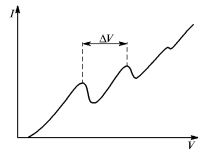
\includegraphics[width=4cm, height=3cm]{5.2.1-1}
\end{wrapfigure}		
	

В результате на приборах наблюдается следующая картина, описывающая данное явление: при увеличении потенциала анода ток в лампе вначале растёт, подобно тому как это происходит в вакуумном диоде (рис. 1). Однако, когда энергия электронов становится достаточной для возбуждения атомов, ток коллектора резко уменьшается. Это происходит потому, что при неупругих соударениях с атомами электроны теряют свою энергию и не могут преодолеть задерживающего потенциала между анодом и коллектором. При дальнейшем увеличении потенциала анода ток коллектора вновь возрастает: электроны, испытавшие неупругие соударения, успевают набрать энергию, достаточную для преодоления задерживающего потенциала.

\subsection{Экспериментальная установка}

\begin{wrapfigure}[12]{r}{0.25\textheight}
	\vspace{-3ex}
	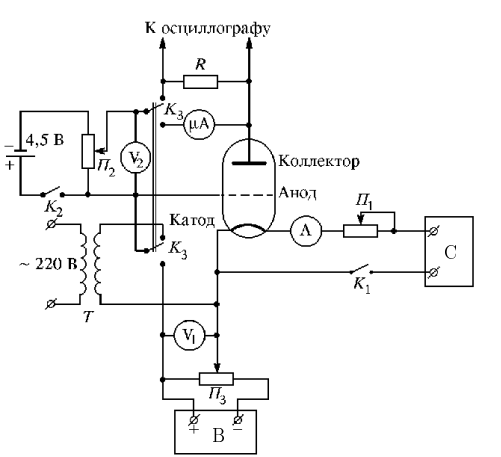
\includegraphics[width=8cm, height=6cm]{5.2.1-2}
\end{wrapfigure}	

Схема экспериментальной установки представлена на рисунке. Для опыта используется трёхэлектродная лампа, заполненная гелием. Источником электронов является вольфрамовый катод, нагреваемый переменным током. В качестве анода используется двойная спираль, окружающая катод. Роль коллектора играет полый металлический цилиндр, соосный с катодом и анодом. Ускоряющее напряжение подается на анод через выпрямитель В. Величина этого напряжения регулируется потенциометром П$_3$ и измеряется вольтметром $V_1$. Величина задерживающего напряжения регулируется потенциометром П$_2$ и измеряется вольтметром $V_2$. Ток через коллектор регистрируется микроамперметром.

	В работе используются два метода: статический и динамический. Для их переключения используется ключ (рис. ниже). Для анализа результатов в динамическом методе используется картинка осциллографа, в статическом - график $I_{\text{к}}(U_{\text{а}})$ 
	
\begin{figure}[H]
	\begin{center}
		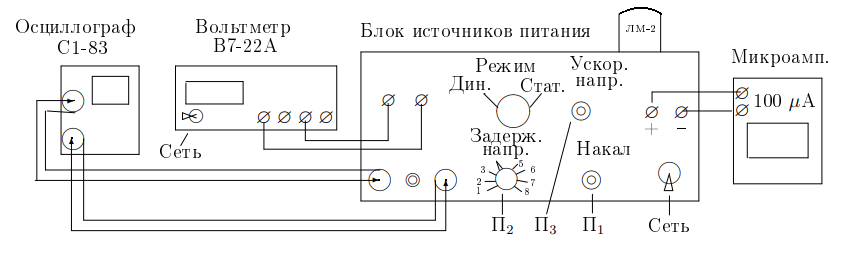
\includegraphics[width=14cm]{5.2.1-3}
	\end{center}
\end{figure}


\section{Результаты измерений и обработка данных}

\subsection{Динамический метод}

$U_2$ - значение запирающего напряжения

\begin{figure}[H]
\begin{minipage}[h]{0.31\linewidth}
\center{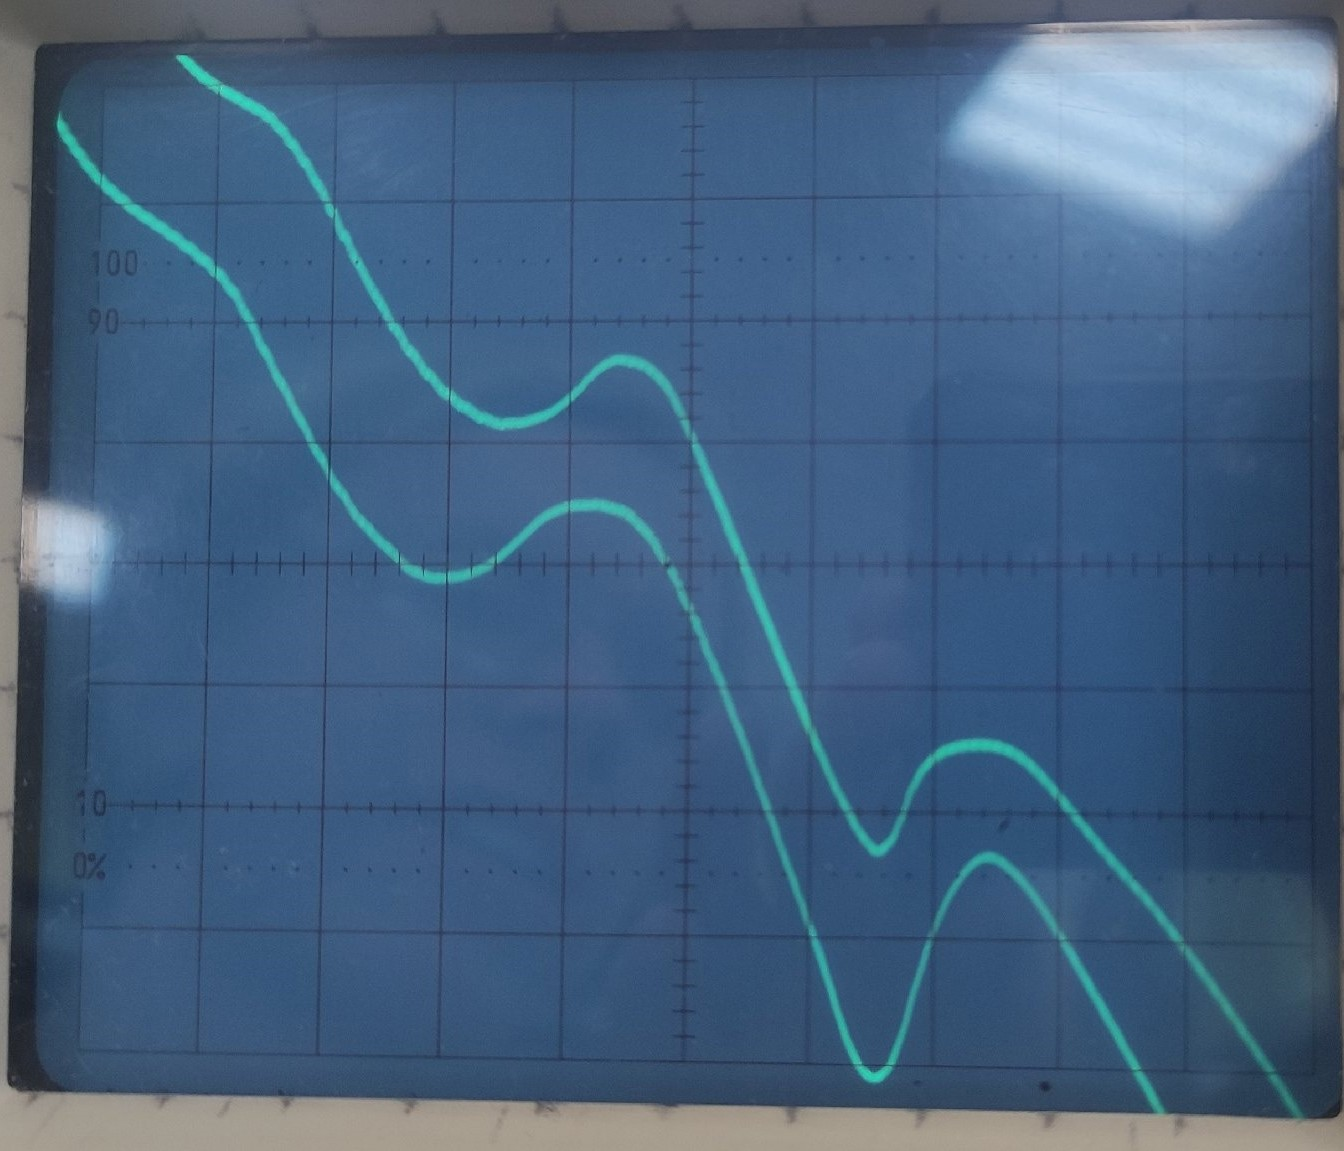
\includegraphics[width=1\linewidth]{5.2.1-4}} 4 В \\
\end{minipage}
\hfill
\begin{minipage}[h]{0.31\linewidth}
\center{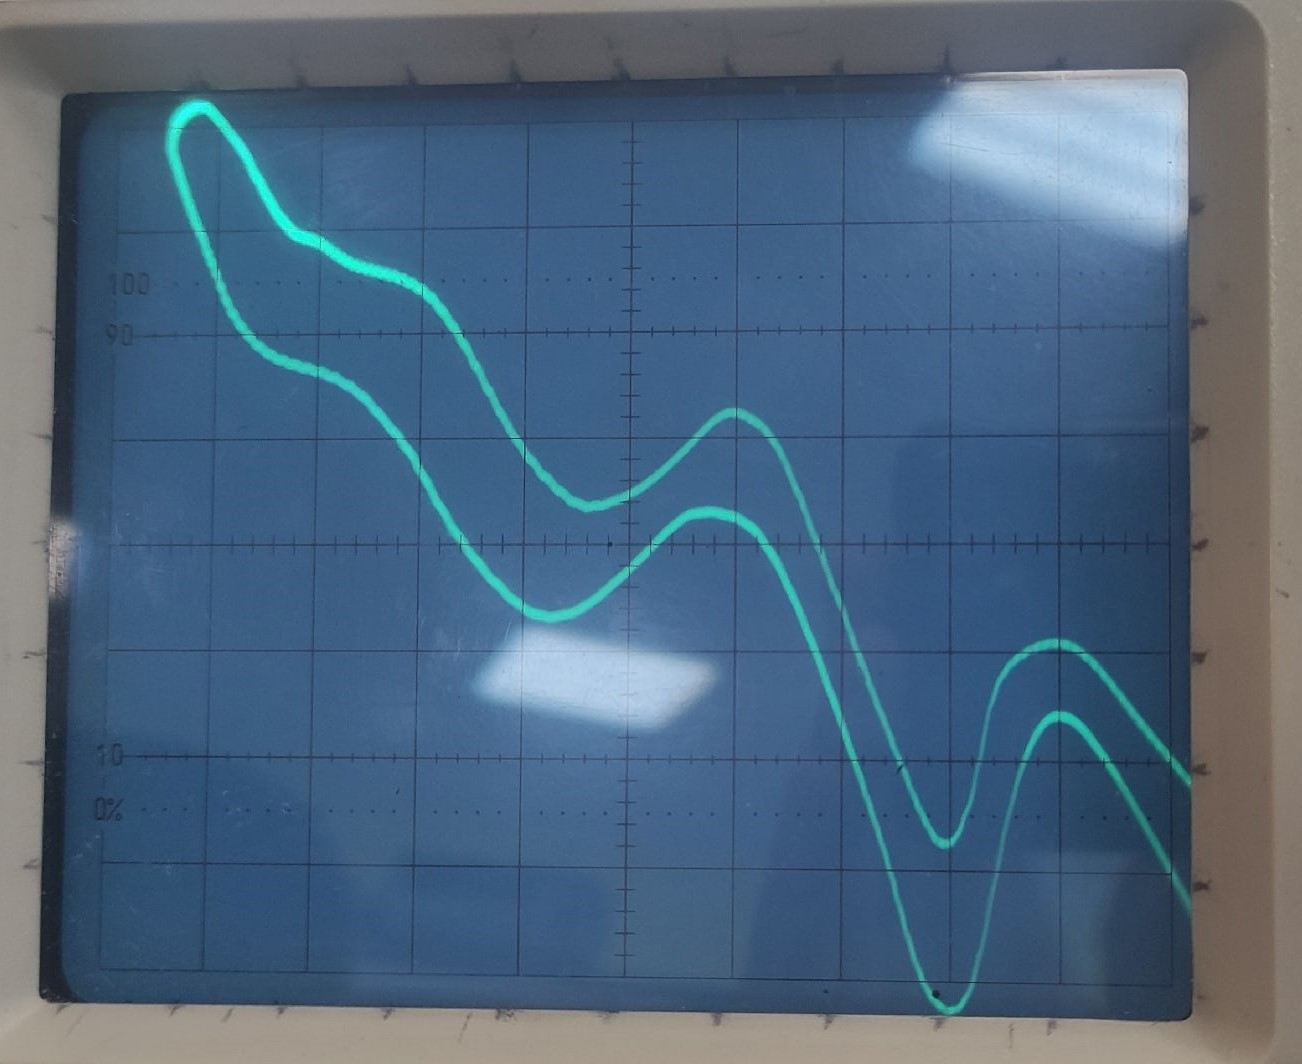
\includegraphics[width=1\linewidth]{5.2.1-5}} \\ 6 В
\end{minipage}
\hfill
\begin{minipage}[h]{0.31\linewidth}
\center{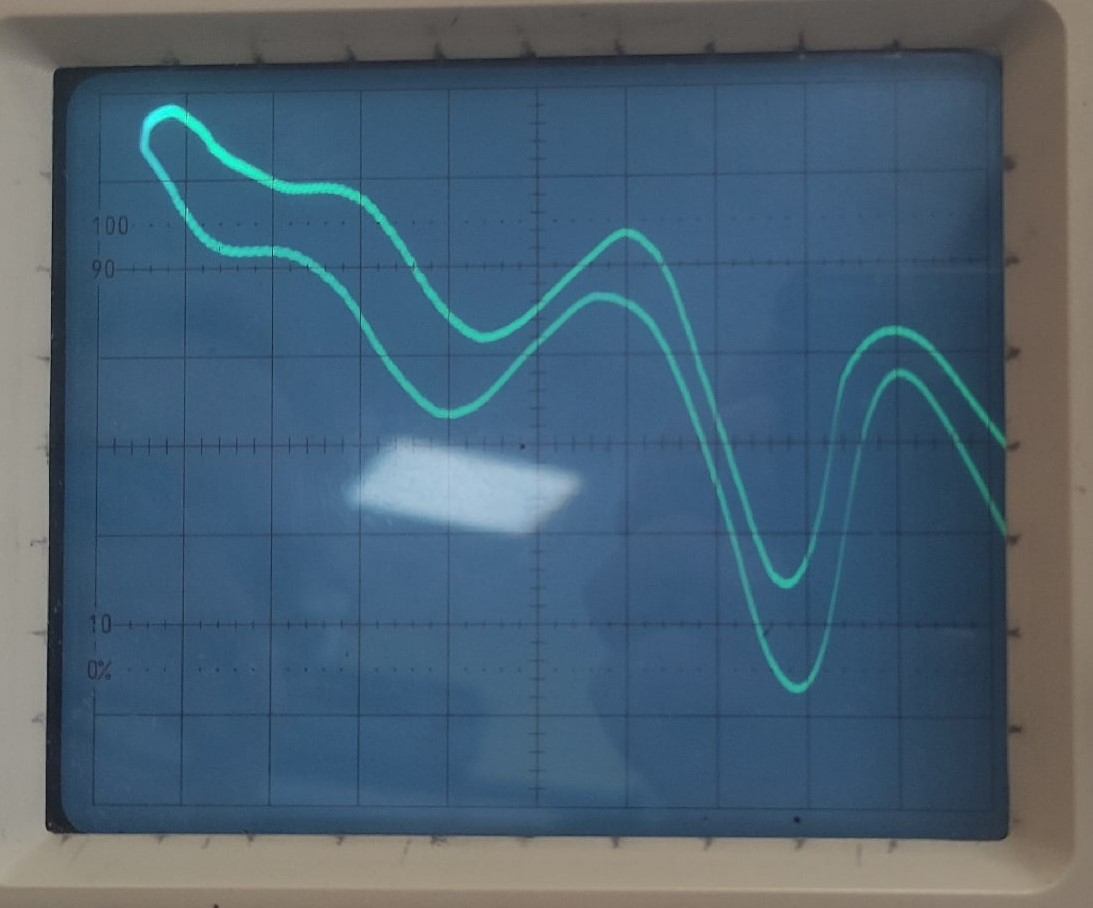
\includegraphics[width=1\linewidth]{5.2.1-6}} \\ 8 В
\end{minipage}
\end{figure}

По картинкам на осциллографе определим расстояния между максимумами и минимумами, внесём данные в таблицу.
 
\begin{center}
\begin{tabular}{|c|c|c|}
\hline 
$U_2$, В & $\Delta{U}^{min}$,В & $\Delta{U}^{max}$,В \\ 
\hline 
4 & 15 & 16 \\ 
\hline 
6 & 16 & 18 \\ 
\hline 
8 & 16 & 18 \\ 
\hline 
\end{tabular} 
\end{center}

\begin{large}
 $\sigma_{\Delta U}$ = 2 В - погрешность измерений $\Delta U$\hfill\break
 
 $\overline{\Delta{U}^{min}} = \frac{\Delta{U}^{min}(U_2 = 4B) + \Delta{U}^{min}(U_2 = 6B) + \Delta{U}^{min}(U_2 = 8B)}{3} = \frac{15 + 16 + 16}{3}B = 15.7 B$ 

$\overline{\Delta{U}^{max}} = \frac{\Delta{U}^{max}(U_2 = 4B) + \Delta{U}^{max}(U_2 = 6B) + \Delta{U}^{max}(U_2 = 8B)}{3} = \frac{16 + 18 + 18}{3}B = 17.3 B$ 

$\sigma \Delta{U}^{min} = \Delta{U}^{min}\sqrt{(\frac{\sigma_{\Delta U}}{\Delta{U}^{min}(U_2 = 4B)})^2 + (\frac{\sigma_{\Delta U}}{\Delta{U}^{min}(U_2 = 6B)})^2 + (\frac{\sigma_{\Delta U}}{\Delta{U}^{min}(U_2 = 8B)})^2} =
\newline
 =15.7\sqrt{(\frac{2}{15})^2 + (\frac{2}{16})^2 + (\frac{2}{16})^2} = 3.5B$

$\sigma \Delta{U}^{max} = \Delta{U}^{max}\sqrt{(\frac{\sigma_{\Delta U}}{\Delta{U}^{max}(U_2 = 4B)})^2 + (\frac{\sigma_{\Delta U}}{\Delta{U}^{max}(U_2 = 6B)})^2 + (\frac{\sigma_{\Delta U}}{\Delta{U}^{max}(U_2 = 8B)})^2} =
\newline
 =17.3\sqrt{(\frac{2}{16})^2 + (\frac{2}{18})^2 + (\frac{2}{18})^2} = 3.5B$
\end{large}

Энергия возбуждения атома гелия : \large{$E = e \Delta{U}^{max} = 17.3 \pm 3.5 эB$}

С учетом порядка погрешности : \large{$E = 17 \pm 4$ эВ}

\subsection{Статический метод}


\begin{tabular}{|c|c|c|c|c|c|c|c|c|c|}
\hline 
$I_\text{к}$, мА & 0,0440 & 0,0634 & 0,1025 & 0.1325 & 0,2120 & 0,2339 & 0,2595 & 0,2976 & 0,2987 \\ 
\hline 
$U_1$, В & 2,77 & 4,08 & 6,49 & 8,09 & 12,69 & 14,13 & 15,82 & 19,3 & 21,55 \\ 
\hline 
$I_\text{к}$, мА & 0.2819 & 0.2619 & 0.2418 & 0.2213 & 0.2325 & 0.2623 & 0.2955 & 0.3181 & 0.3411 \\ 
\hline 
$U_1$, В & 22.49 & 22.76 & 22.92 & 23.39 & 24.58 & 26.00 & 27.80 & 28.84 & 29.98 \\ 
\hline
$I_\text{к}$, мА & 0.3670 & 0.3920 & 0.4191 & 0.4351 & 0.4508 &0.4523 & 0.4394 & 0.4292 & 0.4253 \\
\hline
$U_1$, В & 31.17 & 32.41 & 33.94 & 34.97 & 36.84 & 38.32 & 39.97 & 41.40 & 42.71 \\
\hline 
$I_\text{к}$, мА & 0.4247 & 0.4276 & 0.4374 & 0.4541 & 0.4953 & 0.5425 & & & \\
\hline
$U_1$, В & 43.95 & 45.45 & 46.86 & 49.14 & 53.22 & 57.95 & & & \\
\hline
\end{tabular} 
\begin{center}
\textit{Запирающее напряжение 4 В}
\end{center}

\begin{tabular}{|c|c|c|c|c|c|c|c|c|c|}
\hline 
$I_\text{к}$, мА & 0,0136 & 0,0411 & 0,0688 & 0,1167 & 0,1478 & 0,1758 & 0,1993 & 0,2258 & 0,2455 \\ 
\hline 
$U_1$, В & 2,20 & 4,32 & 6,17 & 8,68 & 10,32 & 11,94 & 13,38 & 15,07 & 16,31 \\ 
\hline 
$I_\text{к}$, мА & 0,2708 & 0,2859 & 0,2860 & 0,2808 & 0,2605 & 0,1974 & 0,2459 & 0,1715 & 0,1541 \\ 
\hline 
$U_1$, В & 18,12 & 19,97 & 21,38 & 22,34 & 23,23 & 23,51 & 23,37 & 23,75 & 24,97 \\ 
\hline 
$I_\text{к}$, мА & 0,1595 & 0,1763 & 0,2123 & 0,2445 & 0,2658 & 0,3031 & 0,3291 & 0,3542 & 0,3722 \\ 
\hline 
$U_1$, В & 25,65 & 26,49 & 27,83 & 29,18 & 30,24 & 31,88 & 33,19 & 34,45 & 35,60 \\ 
\hline 
$I_\text{к}$, мА & 0,3819 & 0,3801 & 0,3675 & 0,3551 & 0,3432 & 0,3354 & 0,3339 & 0,3376 & 0,3474 \\ 
\hline 
$U_1$, В & 37,33 & 39,18 & 40,52 & 42,03 & 43,49 & 45,41 & 48,81 & 48,09 & 49,78 \\ 
\hline 
$I_\text{к}$, мА & 0,3636 & 0,4061 & 0,4402 & • & • & • & • & • & • \\ 
\hline 
$U_1$, В & 52,01 & 56,41 & 62,09 & • & • & • & • & • & • \\ 
\hline 
\end{tabular} 
\begin{center}
\textit{Запирающее напряжение 6 В}
\end{center}

\begin{tabular}{|c|c|c|c|c|c|c|c|c|c|}
\hline 
$I_\text{к}$, мА & 0,0091 & 0,0342 & 0,0622 & 0,1345 & 0,1772 & 0,2151 & 0,2518 & 0,2601 & 0,2721 \\ 
\hline 
$U_1$, В & 3,88 & 5,81 & 7,66 & 11,34 & 13,74 & 16,07 & 18,49 & 19,22 & 20,61 \\ 
\hline 
$I_\text{к}$, мА & 0,2703 & 0,2617 & 0,2423 & 0,1413 & 0,1102 & 0,0991 & 0,1012 & 0,1116 & 0,1313 \\ 
\hline 
$U_1$, В & 22,19 & 23,00 & 23,72 & 23,99 & 24,49 & 25,21 & 26,66 & 27,61 & 28,51 \\ 
\hline 
$I_\text{к}$, мА & 0,1626 & 0,1983 & 0,2283 & 0,2535 & 0,2781 & 0,3045 & 0,3134 & 0,3098 & 0,2943 \\ 
\hline 
$U_1$, В & 29,61 & 30,97 & 32,32 & 33,39 & 34,54 & 36,66 & 38,50 & 39,33 & 41,15 \\ 
\hline 
$I_\text{к}$, мА & 0,2825 & 0,2737 & 0,2558 & 0,2488 & 0,2458 & 0,2504 & 0,2790 & 0,3211 & 0,3280 \\ 
\hline 
$U_1$, В & 42,71 & 43,75 & 45,86 & 47,28 & 48,60 & 50,50 & 54,68 & 60,79 & 63,50 \\ 
\hline 
\end{tabular} 
\begin{center}
\textit{Запирающее напряжение 8 В}
\end{center}


\begin{figure}[H]
	\begin{center}
		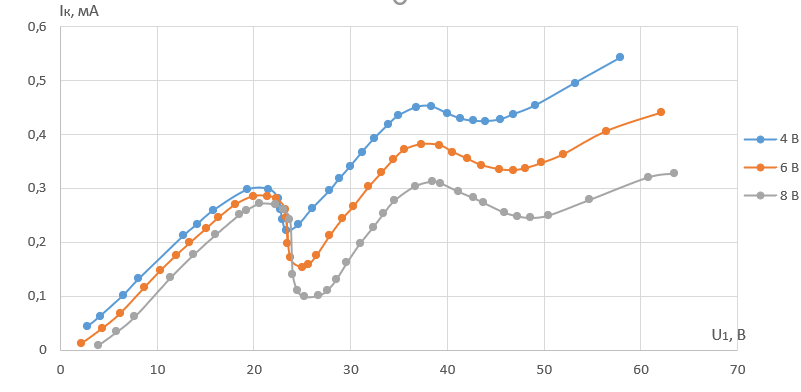
\includegraphics[width=14cm]{5.2.1-7}
	\end{center}
\end{figure}

По графикам определим расстояние между максимумами. Для этого на имеющуюся сетку более точную для уменьшения погрешности.

\begin{center}
\begin{large}
\begin{tabular}{|c|c|c|c|}
\hline 
$U_2$, В & 4 & 6 & 8 \\ 
\hline 
$\Delta U$, В & $18 \pm 1$ & $17 \pm 1$ & $17 \pm 1$ \\ 
\hline 
\end{tabular} 
\end{large}
\end{center}

По формулам, аналогичным используемым в п. 2.1, найдём $\overline{\Delta U}$ и оценим её погрешность. Получим :

\begin{large}
$\overline{\Delta U} = 17,3 \pm 1.7$ В
\end{large}

Тогда энергия возбуждения : \begin{large} E = $17.3 \pm 1.7$ эВ \end{large}

\section{Обсуждение результатов и выводы}

В ходе работы мы получили значения энергии возбуждения атома гелия двумя способами: динамическим и статическим.

\begin{large}
$E^{din} = 17 \pm 4$ эВ

$E^{st} = 17.3 \pm 1.7$ эВ
\end{large} 
 
Полученные значения оказались довольно близкими друг другу, и в пределах погрешностей, их можно считать равными.

Полученные значения оказались близки к энергии возбуждения атома неона (табличное значение 16,8 эВ)
\end{document}